\chapter{Test Automation e Continuous Testing}

\section{Software Quality Assurance}

La \textbf{Software Quality Assurance} (SQA) è definita come l'insieme di attività sistematiche che forniscono evidenza dell'adeguatezza all'uso (\emph{fitness}) del prodotto software complessivo.

I termini principali della definizione sono:

\begin{itemize}
    \item \textbf{Systematic activities}: indica la presenza di un \textbf{processo} regolato;
    \item \textbf{Providing evidence}: indica la presenza di \textbf{punti di controllo} per dimostrare la conformità;
    \item \textbf{Fitness}: indica la presenza di \textbf{obiettivi misurabili} da raggiungere.
\end{itemize}


\begin{notaprof}
Un processo di SQA è un insieme di piani e attività per il monitoraggio e il controllo del processo di sviluppo software. Il suo scopo è assicurarsi che i vari attori stiano lavorando nella giusta direzione.
\end{notaprof}

Gli obiettivi della SQA sono fornire sufficiente confidenza che il prodotto software:

\begin{itemize}
    \item soddisfi le sue specifiche;
    \item sia utilizzabile nel contesto considerato;
    \item venga sviluppato secondo le modalità stabilite.
\end{itemize}

Le componenti della SQA includono \textbf{software testing}, \textbf{quality control}, \textbf{software configuration management}, standard, procedure, convenzioni e specifiche.

\begin{notaesame}
Il \textbf{software testing} è solo una delle componenti della SQA. Le attività di testing devono essere sempre collegate a un piano di qualità più ampio che definisce cosa significhi qualità per quello specifico progetto.
\end{notaesame}

\begin{figure}[htbp]
    \centering
    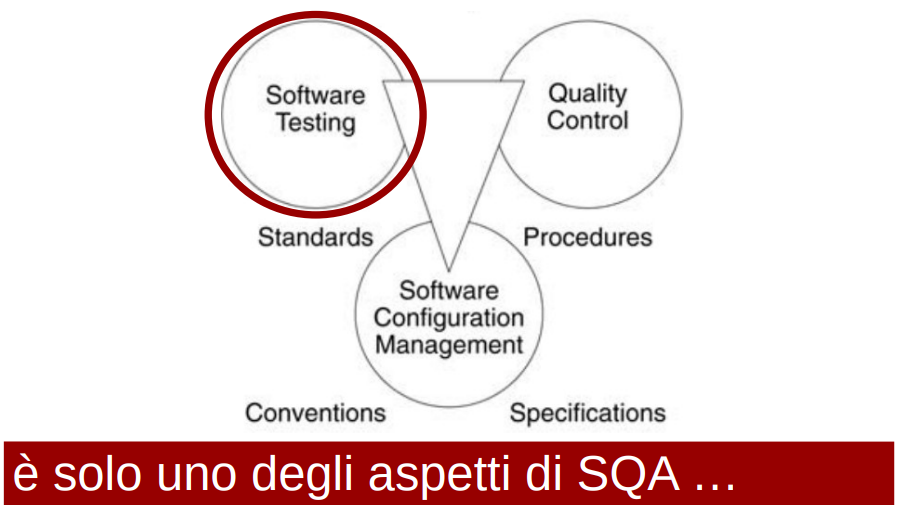
\includegraphics[width=0.62\textwidth]{img/DeAngelis/03_Automatic&ContinuosTesting/SQA_testing}
    \caption{Il software testing come una delle componenti della Software Quality Assurance: la figura evidenzia che il testing si inserisce in un quadro più ampio che comprende anche quality control, procedure e software configuration management.}
    \label{fig:lez8-sqa-testing}
\end{figure}

\section{Esempio \texttt{myBuggyFact}}

Nelle slide viene mostrata una funzione ricorsiva per il calcolo del fattoriale:

\begin{verbatim}
int myBuggyFact(int p){
    int result = abs(p);
    if (result > 1){
        int next = result - 1;
        result = result * myBuggyFact(next);
    }
    return result;
}
\end{verbatim}

Poiché il parametro in ingresso è un \texttt{int}, testare esaustivamente la procedura richiederebbe \(2^{32}\) possibili test.

\begin{notaprof}
Rintracciare l'input che fa fallire la funzione tra \(2^{32}\) possibilità, senza supporto automatico, equivale a cercare un ago in un pagliaio. L'automazione è quindi fondamentale per eseguire validazioni in tempi ragionevoli.
\end{notaprof}

\section{Automated Testing}

L'\textbf{automated testing} consiste nello svolgimento delle attività di test principalmente tramite infrastrutture o framework di supporto.

Le attività che possono essere automatizzate includono:

\begin{itemize}
    \item esecuzione dei test;
    \item generazione dei report;
    \item selezione dei casi di test da eseguire;
    \item prioritizzazione dei test;
    \item valutazione della validità o bontà di un insieme di casi di test.
\end{itemize}

L'automated testing si contrappone al \textbf{manual testing}, in cui i test sono svolti da tester umani, membri del team di QA o utenti finali.

\begin{notaprof}
I framework automatici migliorano efficienza ed efficacia del testing: riducono costi e durata delle fasi di test, aumentano la ripetibilità degli esperimenti, migliorano l'attendibilità statistica e producono una documentazione più leggibile delle failure.
\end{notaprof}

\section{Continuous Testing e Continuous Integration}

Il \textbf{Continuous Testing} consiste nell'integrare i processi di software testing con:

\begin{itemize}
    \item ambienti di sviluppo;
    \item strumenti di build;
    \item sistemi di versioning.
\end{itemize}

I test vengono eseguiti automaticamente sulla versione corrente del sistema, sia in configurazioni locali allo sviluppo sia in ambienti simili a quelli di produzione.

\begin{notaprof}
Nel Continuous Testing lo sviluppo non si interrompe: a ogni evoluzione significativa della code-base si attiva una catena automatica di controlli.
\end{notaprof}

Gli sviluppatori non devono avviare esplicitamente i test remoti, ma ricevono notifiche asincrone sui risultati.

\begin{notaslide}
Le slide evidenziano la necessità di policy per selezione, prioritizzazione e orchestrazione dei casi di test da eseguire.
\end{notaslide}

Il ciclo \textbf{CI + CT} può essere sintetizzato così:

\[
\text{Source control} \rightarrow \text{Trigger} \rightarrow \text{Build server} \rightarrow \text{Report} \rightarrow \text{Development}
\]

Il \textbf{build server} si occupa di:

\begin{itemize}
    \item configurare un ambiente tipo;
    \item eseguire la build del sistema;
    \item eseguire i casi di test.
\end{itemize}

\begin{figure}[htbp]
    \centering
    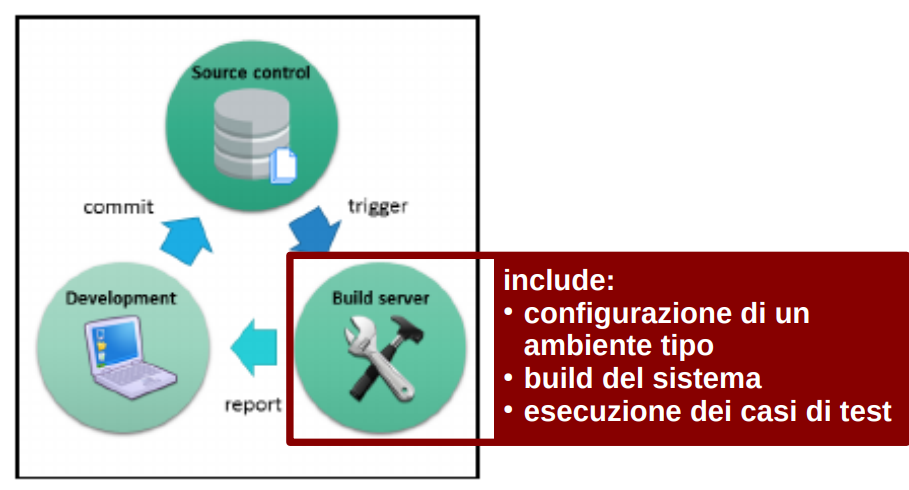
\includegraphics[width=0.68\textwidth]{img/DeAngelis/03_Automatic&ContinuosTesting/CICT}
    \caption{Schema concettuale di integrazione tra Continuous Integration e Continuous Testing: il build server configura l'ambiente, costruisce il sistema ed esegue automaticamente i casi di test.}
    \label{fig:lez8-ci-ct}
\end{figure}

\section{Git e Source Control}

\textbf{Git} è un sistema di controllo versione open-source e distribuito.

\begin{notaprof}
Nel progetto si utilizza un approccio basato su \textbf{blessed repository}. Lo sviluppatore crea un \textbf{fork} del repository principale, lavora sul proprio repository locale, esegue il \textbf{push} sul fork remoto e propone l'integrazione tramite \textbf{Pull Request} all'integration manager.
\end{notaprof}

I concetti principali sono:

\begin{itemize}
    \item \textbf{local repository}: copia locale del repository;
    \item \textbf{fork}: copia personale del repository remoto;
    \item \textbf{push}: invio delle modifiche al repository remoto;
    \item \textbf{pull request}: richiesta di integrazione delle modifiche;
    \item \textbf{blessed repository}: repository principale;
    \item \textbf{integration manager}: responsabile dell'integrazione delle modifiche.
\end{itemize}

\begin{notaesame}
I controlli di qualità e la Continuous Integration vengono tipicamente attivati quando si apre una Pull Request o quando si effettua un push sul repository.
\end{notaesame}

\section{Maven}

\textbf{Maven} è un sistema di build sviluppato da Apache Software Foundation, rivolto principalmente ad ambienti Java.

Uno dei suoi ruoli principali è la gestione delle dipendenze.

\begin{notaprof}
La caratteristica fondamentale di Maven è la gestione esplicita e transitiva delle dipendenze. Lo sviluppatore dichiara le librerie necessarie e le loro versioni; Maven scarica automaticamente tali librerie e anche le dipendenze indirette richieste.
\end{notaprof}

Un progetto Maven segue in genere una struttura standard di directory, pensata per distinguere chiaramente il codice applicativo, i test e i risultati prodotti dalla build.

La directory \texttt{target} contiene tipicamente i risultati della build.

Il file principale di configurazione è il \texttt{pom.xml}, che raccoglie le informazioni fondamentali del progetto e le direttive necessarie per gestirne dipendenze, build, test e deploy.

Le principali fasi Maven sono:

\begin{itemize}
    \item \texttt{validate};
    \item \texttt{compile};
    \item \texttt{test};
    \item \texttt{package};
    \item \texttt{integration-test};
    \item \texttt{verify};
    \item \texttt{install};
    \item \texttt{deploy};
    \item \texttt{clean};
    \item \texttt{site}.
\end{itemize}

\begin{notaesame}
Le fasi Maven sono sequenziali. Un errore in una fase, ad esempio un test fallito durante la fase \texttt{test}, comporta il fallimento dell'intero processo di build.
\end{notaesame}

\section{JUnit}

\textbf{JUnit} è un framework open-source per l'implementazione di programmi di test in Java. È essenziale per rendere la build \textbf{self-testing}.

JUnit ha contribuito a rendere il test, soprattutto quello di unità, una parte centrale della programmazione e ha favorito tecniche come il \textbf{Test-Driven Development} (TDD).

Gli obiettivi principali di JUnit sono:

\begin{itemize}
    \item supportare la definizione di casi di test utili;
    \item supportare test ripetibili nel tempo;
    \item ridurre i costi di scrittura dei test tramite pratiche orientate al riuso.
\end{itemize}

\begin{notaesame}
JUnit fornisce l'infrastruttura per scrivere ed eseguire test, ma \textbf{non} decide la strategia di test, \textbf{non} seleziona i valori di input e \textbf{non} indica quali test siano più significativi. Queste decisioni spettano all'ingegnere.
\end{notaesame}

La versione di riferimento per il corso è \textbf{JUnit 4}, che si basa sull'uso di annotazioni per definire e organizzare i casi di test.

\begin{notaslide}
JUnit 5 introduce una maggiore modularità architetturale, permette la composizione esplicita di più runner e distingue tra API per scrivere test e SPI per estendere strategie di scoperta, scelta ed esecuzione dei test.
\end{notaslide}

\section{Annotazioni JUnit 4 e Maven}

In JUnit 4, un caso di test è un metodo pubblico annotato con \texttt{@Test}.

Le annotazioni principali sono:

\begin{itemize}
    \item \texttt{@Test}: identifica un metodo come caso di test;
    \item \texttt{@Before}: metodo eseguito prima di ogni test;
    \item \texttt{@After}: metodo eseguito dopo ogni test;
    \item \texttt{@BeforeClass}: metodo eseguito una sola volta prima di tutti i test della classe;
    \item \texttt{@AfterClass}: metodo eseguito una sola volta dopo tutti i test della classe.
\end{itemize}
\begin{figure}[htbp]
    \centering
    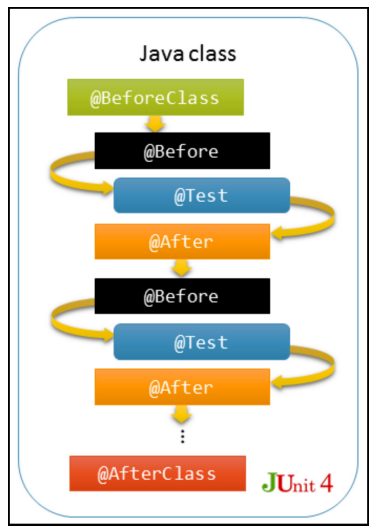
\includegraphics[width=0.25\textwidth]{img/DeAngelis/03_Automatic&ContinuosTesting/JUNIT4}
    \caption{Ciclo di esecuzione di un test in JUnit 4: la figura distingue le operazioni di setup e teardown a livello di classe da quelle eseguite prima e dopo ogni singolo caso di test.}
    \label{fig:lez8-junit4-lifecycle}
\end{figure}

\begin{notaslide}
L'ordine di esecuzione tra più metodi con la stessa annotazione, ad esempio più metodi \texttt{@Before}, non è specificato.
\end{notaslide}

Il flusso logico di esecuzione è:

\[
\texttt{@BeforeClass}
\rightarrow
(\texttt{@Before} \rightarrow \texttt{@Test} \rightarrow \texttt{@After})
\rightarrow
\texttt{@AfterClass}
\]

Affinché Maven riconosca ed esegua automaticamente i test durante la fase \texttt{test}, le classi di test devono rispettare specifici pattern di nomenclatura:

\begin{itemize}
    \item \texttt{Test*};
    \item \texttt{*Test};
    \item \texttt{*Tests};
    \item \texttt{*TestCase}.
\end{itemize}

\begin{notaesame}
Se una classe di test non rispetta i pattern riconosciuti da Maven, può essere ignorata durante la fase di test. In questo caso la CI potrebbe segnalare successo senza aver realmente eseguito quei test.
\end{notaesame}

\section{Framework CI/CD}

Tra i principali framework di Continuous Integration e Continuous Delivery citati nelle slide ci sono:

\begin{itemize}
    \item \textbf{Travis CI};
    \item \textbf{GitHub Actions};
    \item \textbf{GitLab CI/CD};
    \item \textbf{CircleCI}.
\end{itemize}

\begin{notaslide}
Questi framework sono offerti come servizi remoti e prevedono policy e costi di utilizzo. Spesso non ci sono costi per progetti open-source.
\end{notaslide}

\begin{notaesame}
Per i progetti universitari open-source, i limiti degli account gratuiti sono generalmente sufficienti. Non è richiesta una sottoscrizione a pagamento.
\end{notaesame}

Ogni framework richiede una configurazione specifica rispetto al sistema di versioning utilizzato, spesso tramite file di configurazione dedicati.

\section{Visione complessiva e progetto}

La visione complessiva collega \textbf{Git}, \textbf{Maven}, \textbf{JUnit} e un framework di \textbf{CI/CD}.

Il flusso tipico è:

\begin{enumerate}
    \item lo sviluppatore lavora localmente;
    \item usa Maven per compilare e JUnit per testare;
    \item effettua il push sul proprio fork;
    \item apre una Pull Request verso il repository principale;
    \item la Pull Request attiva il server di Continuous Integration;
    \item il server scarica le dipendenze tramite Maven;
    \item il server esegue la build;
    \item il server lancia i test JUnit;
    \item viene prodotto un report di successo o fallimento.
\end{enumerate}

\begin{figure}[htbp]
    \centering
    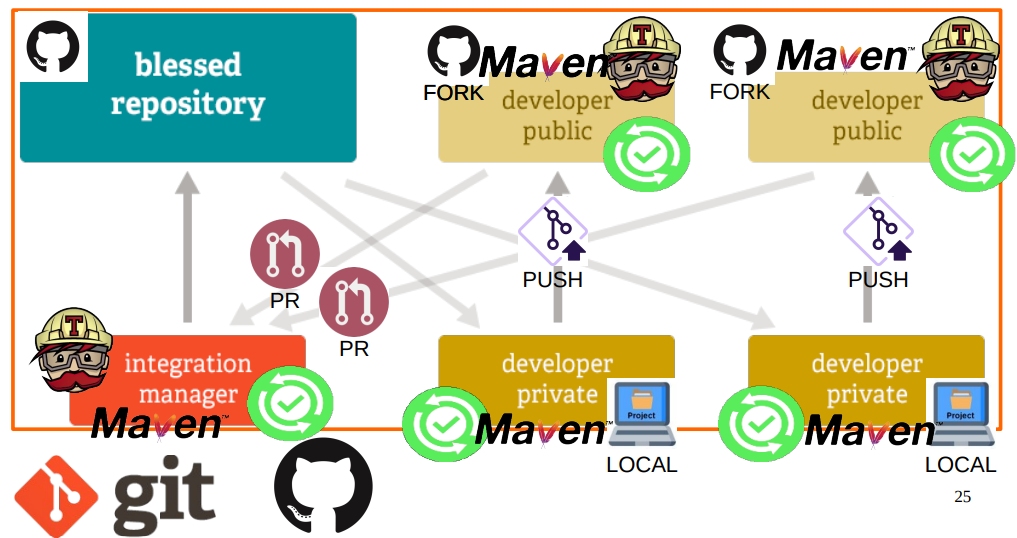
\includegraphics[width=0.72\textwidth]{img/DeAngelis/03_Automatic&ContinuosTesting/CICT_completa}
    \caption{Visione complessiva del flusso di Continuous Integration e Continuous Testing: commit, push, pull request, build automatica ed esecuzione dei test concorrono a mantenere sotto controllo la qualità del software.}
    \label{fig:lez8-ci-ct-overview}
\end{figure}

\begin{notaprof}
L'automazione serve a verificare che il codice non funzioni solo sulla macchina dello sviluppatore, ma anche in ambienti puliti, riproducibili ed eterogenei.
\end{notaprof}

Gli errori da evitare nel progetto sono:

\begin{itemize}
    \item configurare in modo errato il \texttt{pom.xml};
    \item usare nomi di classi di test non riconosciuti da Maven;
    \item lasciare dipendenze mancanti;
    \item avere una build non riproducibile;
    \item non integrare automaticamente i test nella build.
\end{itemize}
